\chapter{Διαδικασία Σχεδίασης και Υλοποίησης} % Main chapter title
\label{chap:Chapter4}  % For referencing the chapter elsewhere, use \ref{Chapter4}

% \epigraph{”Our goals can only be reached through a vehicle of a plan, in which we must fervently believe, and upon which we must vigorously act. There is no other route to success." }{\textit{Pablo Picasso}}
\epigraph{”Οι στόχοι μας μπορούν μόνο να έρθουν εις πέρας με την σχεδιάση ενός καλά οργανωμένου πλάνου, στο οποίο πρέπει επίμονα να πιστεύουμε, και το οποίο με σθένος πρέπει να πράτουμε. Δεν υπάρχει άλλος δρόμος για την επιτυχία." }{\textit{Pablo Picasso}}

Στο παρόν κεφάλαιο περιγράφεται η διαδικασία σχεδιασμού και υλοποίησης του \Abbr{MoCap} με χρήση drone swarm συστήματος, που συσχετίζεται η παρούσα διπλωματική. 

Μία high-level προσέγγιση, θα μπορούσε να διαχωρίζει το σύστημα σε τρία διακριτά
υποσυστήματα. Αρχικά το optical, του οποίου αρμοδιότητα είναι το detection, το tra\-cking, καθώς και η εκτίμηση
του range ή γωνίας του αντικειμένου από την camera. Δεύτερο, η λήψη των πληροφοριών από τους αισθητήρες ώστε να προσεγγιστεί η θέση του ίδιου
του drone. Τέλος, ο συνδυασμός των δύο παραπάνω μερών και η χρήση κατάλληλης localization τεχνικής για να βρεθεί η θέση του αντικειμένου
στο \Abbr{3D} χώρο.

Πριν γίνει αναφορά καθενός από τα υποσυστήματα που σχεδιάστηκαν, στην \Fig{high-level-system-block-diagram} παρουσιάζεται ένα block diagram του γενικού συστήματος, το οποίο αποτελείται από τα worker nodes - δουλειά των οποίων είναι η ανίχνευση του αντικειμένου και εκτίμηση της απόστασης του από αυτά - τα οποία αποστέλλουν στον master του συστήματος όλες τις πληροφορίες που έχουν συλλέξει και είναι αυτός που α\-να\-λα\-μβά\-νει τον προσδιορισμό της θέσης τελικά του object.

% Image
\FigCaptLabelBasedURL{../Photos/High-level-top-diagram.drawio.png}%
{High level system block diagram}%{}
{high-level-system-block-diagram}%
<1>

%----------------------------------------------------------------------

\section{Τεχνολογίες και εργαλεία} \label{sec:design-tools}
Αρχικά θα αναφερθούν συνοπτικά οι τεχνολογίες στις οποίες έγινε επιλογή να επιλυθεί το πρόβλημα,
όπως επίσης και τα εξαρτήματα/αισθητήρια όργανα καθώς και τα λογισμικά τα οποία χρησιμοποιήθηκαν. 
Συνοπτικά, μπορεί να αναφερθεί ότι το σύνολο της υλοποίησης\footnote{Η οποία μπορεί να βρεθεί ως open source project διαθέσιμη στον εξής σύνδεσμο \cite{thesis-project-location}} αποτελείται από κώδικα C++, Bash scripts, Matlab scripts και ROS configuration files.

%----------------------------------------------------------------------

\subsection{Embedded Linux System}
Δύο πολύ δημοφιλείς επιλογές στον χώρο των ενσωματωμένων συστημάτων - ως κεντρικές μονάδες επεξεργασίας - είναι οι πλακέτες Raspberry Pi που κατασκευάζονται από την Raspberry Pi Foundation σε συνεργασία με την Broadcom, καθώς και οι πλακέτες Jetson της Nvidia. Στην \Fig{embedded-linux-systems} ως παράδειγμα παρουσιάζονται ενδεικτικά μία εκδοχή από την κάθε οικογένεια, ενώ στον \Tabl{raspberry-pi-specs} και \Tabl{jetson-nano-specs} τα τεχνικά χαρακτηριστικά της εκάστοτε πλακέτας ως αρχικό σημείο αναφοράς. 

\begin{figure} [H]
	\centering
	% -----------------
    \begin{minipage}{.5\textwidth}
      \centering
      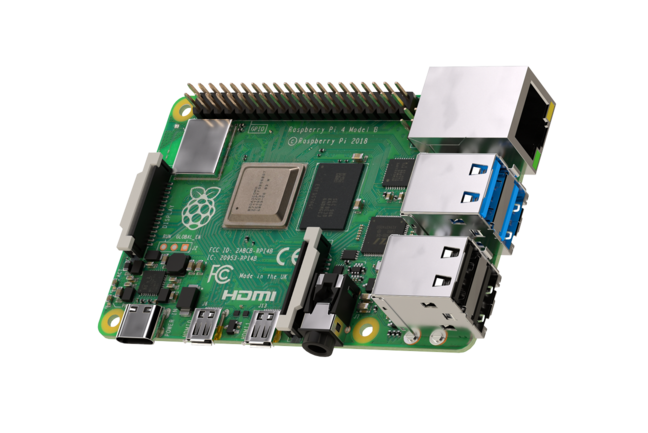
\includegraphics[width=\linewidth]{../Images/Design-Implementation/raspberry-pi-4.png}\\
      {(a) Raspberry Pi 4 \URI{https://www.hellasdigital.gr/go-create/raspberry-and-accessories-el/raspberry-pi/raspberry-pi-4-4gb-ram/}}
    \end{minipage}%
    % -----------------
    \begin{minipage}{.5\textwidth}
      \centering
      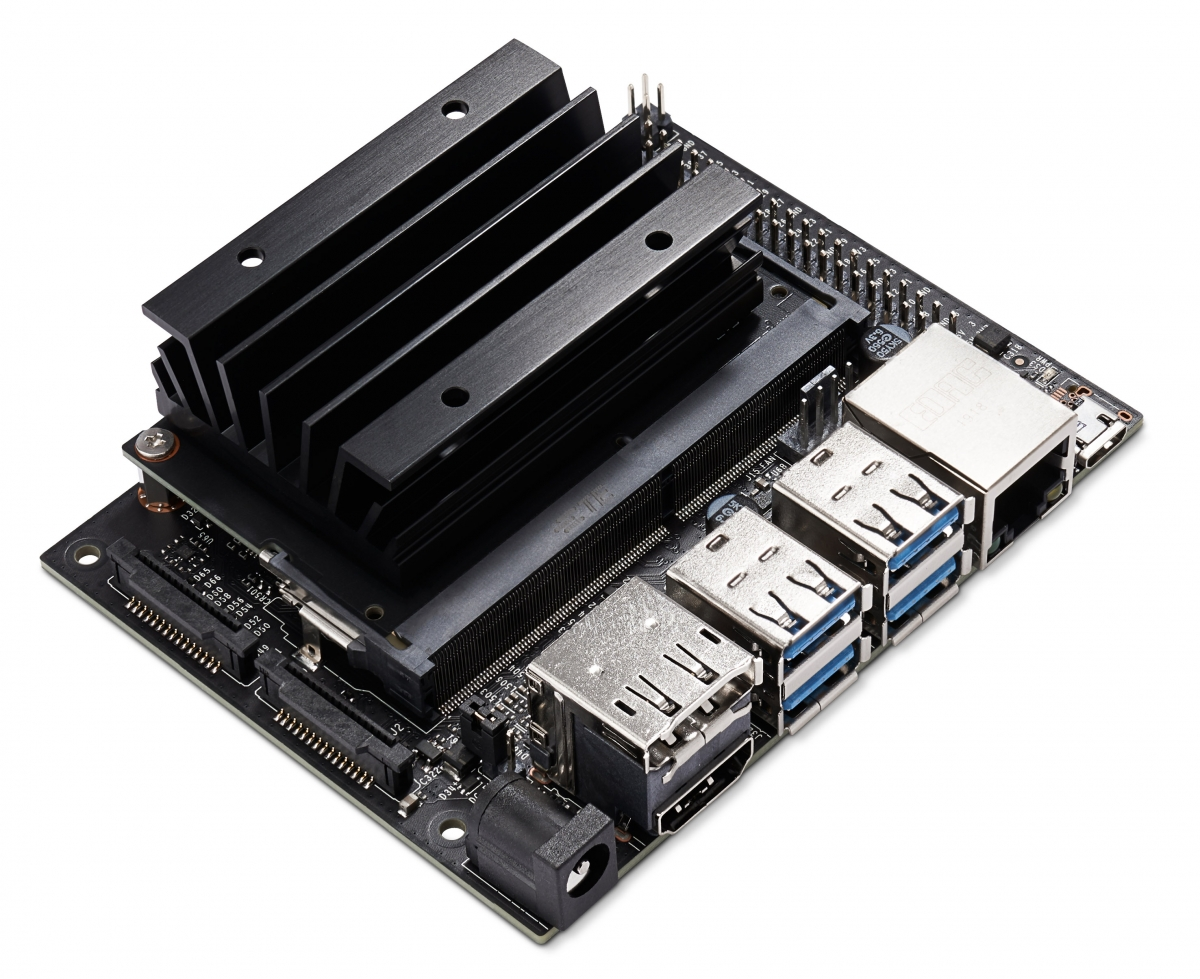
\includegraphics[width=.9\linewidth]{../Images/Design-Implementation/jetson-nano.jpeg}\\
      {(b) Jetson Nano \URI{https://www.hellasdigital.gr/computers/accessories/nvidia-jetson-nano-developer-kit/}}
	\end{minipage}
	% -----------------
    \hfill \break
    \decoRule
    \CaptionBasedwithURL{Υποψήφια Embedded Linux Systems για την υλοποίηση} %\CaptionBasedwithURL{Possible Embedded Linux Systems} 
    \label{fig:embedded-linux-systems}
\end{figure}

Και οι δύο επιλογές αποτελούνται από έναν ARM αρχιτεκτονικής Central Processing Unit (\Abbr{CPU}), ενώ στις Jetson βρίσκεται επιπρόσθετα και ένα Graphics Processing Unit (\Abbr{GPU}) που μπορεί να χρησιμοποιηθεί σε ενσωματωμένα με μεγάλες ανάγκες επεξεργασίας (όπως αυτά που σχετίζονται με εικόνα/βίντεο).

\begin{table}[H]
    \caption[]{Raspberry Pi 4 Model B Specifications}
    \label{tab:raspberry-pi-specs}
    \centering
    \resizebox{.63\textwidth}{!}{
        \begin{tabular}{ll}
            \hline
            \textbf{Feature} & \textbf{Value}  \\
            \hline
                Processor & \Centerstack{Broadcom BCM2711, Quad core Cortex-A72 \\(ARM v8) 64-bit SoC @ 1.5GHz }\\
                Memory & 8GB LPDDR4-3200 SDRAM \\
                Storage & External Micro-SD \\  
                Power & 5V DC (maximum 3A), 5-15Watt \\
                Cost & $\sim$100 €\\
                Weight & 46 grams (without case), 99 grams (with case) \\
                Peripherals & GPIO, I2C, SPI, UART \\
                \hline
        \end{tabular}
    }
  \end{table}

  Στην συγκεκριμένη διπλωματική επιλέχθηκε η ανάπτυξη του συστήματος να γίνει σε Raspberry Pi 4 boards - λόγω του ελάχιστα μικρότερου κόστους καθώς και μάζας τους - έχοντας μελλοντικά την επιλογή για migration ενός ή περισσότερων κόμβων του συστήματος σε Jetson boards, αν κριθεί αυτή η ανάγκη, για λόγους σχετικούς με την ταχύτερη επεξεργασία των δεδομένων.

  \begin{table}[H]
        \caption[]{Jetson Nano Developer Kit Specifications}
        \label{tab:jetson-nano-specs}
        \centering
        \resizebox{.63\textwidth}{!}{
            \begin{tabular}{ll}
                \hline
                \textbf{Feature} & \textbf{Value}  \\
                \hline
                    CPU & Quad-core ARM Cortex-A57 MPCore processor\\
                    GPU & \Centerstack{NVIDIA Maxwell architecture with 128 NVIDIA\\ CUDA® cores} \\
                    Memory & 4 GB 64-bit LPDDR4; 25.6 gigabytes/second \\
                    Storage & External Micro-SD \\  
                    Power & 5V DC, 5-10Watt \\
                    Cost & $\sim$120€\\
                    Weight & 250 grams (without case)\\
                    Peripherals & GPIO, I2C, I2S, SPI, UART \\
                    \hline
            \end{tabular}
        }
      \end{table}

%----------------------------------------------------------------------

\subsection{ROS} \label{sec:ROS}
Συνδετικός κρίκος των υποσυστημάτων είναι το open-source middleware Robot Operation System (\Abbr{ROS}) \cite{ros} το οποίο 
πε\-ρι\-λα\-μβά\-νει ένα εκτενές σύνολο εργαλείων, βιβλιοθηκών και συ\-μβά\-σεων. Τα πακέτα του οποίου χρησιμοποιούνται για την
λήψη και φιλτράρισμα από τους αισθητήρες των πληροφοριών, επικοινωνία μεταξύ των drone όπως τέλος και 
όποια τρι\-σδιά\-στα\-τη απεικόνιση χρειάζεται.

Μεγάλο πλεονέκτημα του \Abbr{ROS} είναι η ύπαρξη των packages. Τα packages είναι δια\-κρι\-τά αυτόνομα κομμάτια κώδικα τα οποία περικλείουν μία συχνά επαναλαμβανόμενη λογική, συνεπώς μπορούν να χρησιμοποιηθούν αυτούσια - με πολύ εύκολο τρόπο - σε διαφορετικές εφαρμογές χωρίς να υπάρχει η ανάγκη να κάνουμε \textit{reinvent the wheel} κάθε φορά, πετυχαίνοντας με αυτό τον τρόπο το rapid prototyping and testing ενός συστήματος καθώς και την αποφυγή δημιουργίας boilerplate κώδικα δίνοντας έμφαση περισσότερο στο main logic του εκάστοτε συστήματος. 

Το \Abbr{ROS} στην πραγματικότητα είναι ένα meta-operating system, με αποτέλεσμα να χρειάζεται να τρέχει σε ένα πρωτεύον Operating System (\Abbr{OS}), με την μεγαλύτερη συμβατότητά να παρέχεται από διανομές Ubuntu Linux. 

Σημαντικές πηγές που χρησιμοποιήθηκαν για την εκμάθηση του \Abbr{ROS} ήταν κυρίως το documentation του \cite{ros-doc}, καθώς και κάποια από τα external tutorials τα οποία προτείνονται στην παραπάνω σελίδα.

%----------------------------------------------------------------------

\subsection{Λειτουργικό σύστημα}
Από την στιγμή που επιλέχθηκε να γίνει χρήση του \Abbr{ROS} - που όπως αναφέρθηκε στη \Sect{ROS} προτείνεται ο συνδυασμός του με Ubuntu Linux - έγινε ε\-γκα\-τά\-στα\-ση στο Raspberry Pi η ειδικά σχεδιασμένη για το αυτό έκδοση Ubuntu Linux 20.04.2 64bit version για ΑRM \cite{ubuntu-raspberry} αρχιτεκτονική. Ουσιαστικά όλες οι λειτουργίες της εφαρμογής θα χρησιμοποιούν το Embedded General Purpose Operating System προκειμένου να λειτουργήσουν, το οποίο σημαίνει ότι αυτό θα είναι κυρίως υπεύθυνο για το scheduling, file-system abstraction, networking, etc. 

%----------------------------------------------------------------------

\subsection{OpenCV}
Για το οπτικό σκέλος χρησιμοποιήθηκε η ανοιχτού κώδικα βιβλιοθήκη OpenCV \cite{opencv}, η οποία αποτελεί την δημοφιλέστερη επιλογή για real-time Computer Vision related εφαρμογές. Ξεκίνησε η ανάπτυξη της στα εργαστήρια της Intel και έχει ήδη διάρκεια ζωής λίγο περισσότερο από δύο δεκαετίες. Για τις ανάγκες της συγκεκριμένης ε\-ργα\-σίας χρησιμοποιήθηκε η έκδοση της 4.2.0. Όμοια με το \Abbr{ROS} και για την εκμάθηση του \Abbr{OpenCV}, καθοριστικό ρόλο συνέβαλε η κατανόηση του επίσημου documentation της βιβλιοθήκης \cite{opencv-4-2-0-doc}.

%----------------------------------------------------------------------

\subsection{Κάμερα}
Σχετικά με την κάμερα, ήταν ανάγκη - όντας πρώτη γενιά του συστήματος -  να επιλεχθεί μία low-cost 1080p camera η οποία θα παρέχει δυνατότητα επιλογής χαμηλότερου resolution για λόγους δοκιμών. Στο πρωτότυπο σύστημα τελικά γίνεται χρήση μία 1080p web cameras της Creative \cite{creative-camera} - \Fig{creative-camera} - με δυνατότητες λήψης βίντεο στα 30fps, η οποία συνδέεται μέσω USB στο Raspberry Pi.

% Image
\FigCaptLabelBasedURL{../Images/Design-Implementation/creative-web-cam.jpeg}%
{Η κάμερα που χρησιμοποιήθηκε για τον εντοπισμό και ανίχνευση του αντικειμένου}%{Camera used for ball detection and tracking}
{creative-camera}%
<0.35>%
(https://en.creative.com/p/peripherals/creative-live-cam-sync-1080p)


%----------------------------------------------------------------------

\subsection{GPS} \label{sec:GPS}
Παρόλο που - όπως αναφέρθηκε στο \Chap{thesis-approach} - στο συγκεκριμένο σύστημα μας ενδιαφέρει το relative positioning και όχι το absolute, σκεπτόμενοι ότι στην πραγματικότητα το σύστημα σχεδιάζεται με γνώμονα το να λειτουργεί σε outdoor scenarios\udot ένας άμεσος τρόπος προσδιορισμού της θέσης του κάθε drone είναι με χρήση κάποιου εμπορικού αισθητήρα \Abbr{GPS}. Στην συνέχεια και αφού έχει αποκτηθεί πληροφορία απόλυτης θέσης για το κάθε drone μπορεί - θεωρώντας ένα από αυτά ως αρχή των αξόνων - να γίνει translate των απόλυτων συντεταγμένων ώστε να κρατηθεί μόνο πληροφορία σχετικά με την χωρική τοπολογία του δικτύου.

Συγκεκριμένα, χρησιμοποιείται το \Abbr{GPS} για commercial χρήση ΒΝ-220 \cite{bn-220-gps} - \Fig{bn-220-gps} - το οποίο υπόσχεται εμβέλειας ακρίβειας της τάξης των δύο μέτρων. Πρακτικά, παρόλο που για ένα \Abbr{MoCap} σύστημα αυτή η τιμή είναι απαγορευτική, χρησιμοποιείται στα πρώτα versions, καθαρά αναφορικά με την εξοικείωση του τρόπου επικοινωνίας \Abbr{ROS} - \Abbr{GPS}. Σε επόμενα revisions σκοπός είναι η αντικατάσταση του με \Abbr{RTK}-\Abbr{GPS} που συχνά μπορεί να φέρουν drone για αυτήν την χρήση ώστε να φτάσει η συνολική ακρίβεια εκτίμησης της απόλυτης θέσης στα μερικά εκατοστά. 

Το συγκεκριμένο \Abbr{GPS} συνδέεται με το Raspberry Pi μέσω Universal Asynchronous Receiver-Transmitter (\Abbr{UART}) \cite{uart-protocol} σύνδεσης και χρησιμοποιεί NMEA-0183 \cite{NMEA-0183-packets} πακέτα για την επικοινωνία. 

\FigCaptLabelBasedURL{../Images/Design-Implementation/bn220.png}%
{Το GPS που χρησιμοποιήθηκε}%{GPS module used to estimate position}%
{bn-220-gps}%
<0.28>%
(https://www.google.com/imgres?imgurl=https\%3A\%2F\%2Fimages.jdmagicbox.com\%2Fquickquotes\%2Fimages_main\%2Fb07wwx5jvp-electroprime-bn-220-3-0v-5-0v-ttl-level-gnss-module-gps-glonass-dual-gps-module-antenna-v4b2-181504802-qn443.jpg&imgrefurl=https\%3A\%2F\%2Fwww.justdial.com\%2FELECTROPRIME-BN-220-3-0V-5-0V-TTL-Level-Gnss-Module-GPS-Glonass-Dual-GPS-Module-Antenna-V4B2\%2Fpid-181504802&tbnid=YJcAk2WsHSEZiM&vet=10CF8QMyiOAWoXChMI2M3PyrCA8wIVAAAAAB0AAAAAEAk..i&docid=xDxMDFHprlF2iM&w=500&h=500&itg=1&q=bn-220\%20image&hl=el&client=ubuntu&ved=0CF8QMyiOAWoXChMI2M3PyrCA8wIVAAAAAB0AAAAAEAk)

%----------------------------------------------------------------------

\subsection{IMU}\label{sec:imu}
Ήδη από τη \Sect{Chapter1-1-2} έχει γίνει αναφορά για την σημαντικότητα των \Abbr{IMU}, καθώς αποτελούν τα κύρια αισθητήρια όργανα καθορισμού σε πολλαπλούς άξονες της σχετικής θέσης/κίνησης του drone. Επιλέχθηκε να χρησιμοποιηθεί το \Abbr{IMU} \cite{adafruit-10dof-imu} της Adafruit - \Fig{adafruit-10DoF-imu} - το οποίο παρέχει 10-\Abbr{DoF}, με onboard αισθητήρες ένα τριών αξόνων accelerometer, τριών αξόνων gyroscope, τριών αξόνων magnetometer (compass), ένα barometric pressure/altitude αισθητήρα και δυνατότητα υ\-πο\-λο\-γι\-σμού της θερμοκρασίας.

Θετικό του συγκεκριμένου module είναι ότι όλοι οι παραπάνω αισθητήρες είναι συ\-νδε\-δε\-μέ\-νοι σε ένα κοινό Inter-Integrated Circuit (\Abbr{I2C}) \cite{I2C-protocol} bus, μέσω του οποίου μπορεί πολύ εύκολα να γίνει η διασύνδεση με την επεξεργαστική μονάδα που επιθυμούμε και να πραγματοποιηθεί επικοινωνία. 

% Image
\FigCaptLabelBasedURL{../Images/Design-Implementation/10DoF-Adafruit-IMU.jpeg}%
{Adafruit 10 DoF IMU}%
{adafruit-10DoF-imu}%
<0.28>%
(https://www.banggood.com/10DOF-LSM303-L3G4200D-BMP180-Pressure-Sensor-Barometer-Accelerometer-Magnetometer-Gyroscope-Compass-Gyro-Module-p-1660604.html?utm_source=googleshopping&utm_medium=cpc_organic&gmcCountry=GR&utm_content=minha&utm_campaign=minha-gr-en-pc&currency=EUR&cur_warehouse=CN&createTmp=1&utm_source=googleshopping&utm_medium=cpc_bgs&utm_content=sxxx&utm_campaign=sxxx-pla-gr-en-all-purchase-rm-pc-0720&ad_id=534554931006&gclid=Cj0KCQjwv5uKBhD6ARIsAGv9a-zYv4IDUcaDBSG_7ggf1nlFXmcM6l9fHjUUGiwKJGhUsgZsQ_BVn4YaAkG4EALw_wcB)

%----------------------------------------------------------------------

\subsection{Breakout Board}
Για να λειτουργήσουν τα παραπάνω υποσυστήματα, χρειαζόταν να πραγματοποιηθούν οι κατάλληλες φυσικές διασυνδέσεις. Η απλούστερη εκδοχή θα ήταν να γίνει αυτό με χρήση breadboard, πράγμα όμως που θα πρόσθετε όγκο και βάρος στο τελικό σύστημα, οι οποίοι σε περίπτωση δοκιμών πάνω σε πραγματικά drone να είναι απαγορευτικοί παράγοντες. Συνεπώς, προκειμένου να μπορεί με ευκολία να γίνει η ανάπτυξη του συστήματος, σχεδιάστηκε (στο cad εργαλείο KiCad \cite{KiCad}) και κατασκευάστηκε ένα custom breakout board - το οποίο είναι διαθέσιμο ως open hardware project στο \cite{raspberry-pi-fan-breadkout} - όπως φαίνεται στην \Fig{raspberry-pi-breakout}. Αυτό παρέχει εύκολη πρόσβαση στα GPIO του Raspberry, έξτρα pins για τροφοδοσία στα 5 και 3.3 Volt, pins για τοποθέτηση αισθητήρων - όπως του \Abbr{IMU} - καθώς και mounting holes στα οποία μπορεί να τοποθετηθεί 40x40mm fan για την ψύξη του συστήματος. 

% Image
\FigCaptLabelBasedURL{../Images/Design-Implementation/Rpi-breakout.png}%
{Raspberry Pi breakout}%
{raspberry-pi-breakout}%
<0.4>


%----------------------------------------------------------------------

\subsection{System Overview}
Η ολοκληρωμένη μορφή του πρωτότυπου συστήματος παρουσιάζεται στην \Fig{thesis-system}, ενώ στο \Tabl{thesis-system-bom} μπορούν να βρεθούν συνολικά τα εξαρτήματα που χρησιμοποιήθηκαν μαζί με την κοστολόγηση τους. 

% Image
\FigCaptLabelBasedURL{../Images/Design-Implementation/thesis-system.jpg}
{Το πρώτυπο σύστημα που σχεδιάστηκε στα πλαίσια της διπλωματικής}%{System designed}%
{thesis-system}%
<0.65>

Το σύστημα ζυγίζει $\sim$ 250gr, μία αρχική εκτίμηση κατανάλωσης είναι τα 15 watt και οι εξωτερικές διαστάσεις του είναι 17x7.5x10.5cm.

\begin{table}[H]
    \caption[]{Bill of Materials}
    \label{tab:thesis-system-bom}
    \centering
    \resizebox{0.55\textwidth}{!}{
        \begin{tabular}{ll}
            \hline
            \textbf{Component} & \textbf{Cost}  \\
            \hline
                Raspberry Pi 4 Model B 8GB & \Centerstack{$\sim$ 100 €}\\
                Creative live cam sync 1080p \cite{creative-camera} & \Centerstack{$\sim$ 44 €}\\
                Adafruit 10 DoF IMU \cite{adafruit-10dof-imu} & \Centerstack{$\sim$ 30 €}\\
                BN-220 GPS Module \cite{bn-220-gps} & \Centerstack{$\sim$ 15 €}\\
                Breakout Board with fan \cite{raspberry-pi-fan-breadkout} & \Centerstack{$\sim$ 8 €}\\
                \hline
        \end{tabular}
    }
  \end{table}


% ------------------------------------------------------------------------------------------------------

\section{Environment}
Έχοντας ήδη αναφερθεί σε όλα τα υποσυστήματα που χρησιμοποιούνται, σε αυτό το section θα δοθεί ο τρόπος με τον οποίο διαμορφώθηκαν/προγραμματίστηκαν ώστε να λειτουργούν μεταξύ τους.

%----------------------------------------------------------------------

\subsection{Παραμετροποίηση OS} 
Στο \cite{ubuntu-raspi-intall} βρίσκονται αναλυτικές οδηγίες εγκατάστασης του Ubuntu στο Ra\-spbe\-rry Pi, ανάλογα με το λειτουργικό που ήδη χρησιμοποιούμε. Στην συγκεκριμένη περίπτωση - επειδή η εγκατάσταση έγινε από διανομή Linux - αφού έγινε λήψη του pre-made image του Ubuntu, βρέθηκε το path της SD card στον υπολογιστή, στην οποία έγινε umount, και στην συνέχεια χρησιμοποιήθηκε η εντολή dd για την δημιουργία του bootable μέσου, με τον εξής τρόπο.

\begin{lstlisting}[language=sh, escapechar=@, caption={Create bootable SD from Linux},label=create-bootable-sd-terminal]
    @\color{dkgreen}{\$}@ sudo dd bs=4M @if@=PATH_TO_YOUR_IMAGE_FILE of=PATH_TO_YOUR_SD_CARD status=progress
\end{lstlisting}

Μόλις ολοκληρωθεί η παραπάνω διαδικασία, το λειτουργικό σύστημα είναι έτοιμο προς χρήση. Αφού έγινε update του συστήματος, έγιναν οι εξής παραμετροποιήσεις. Αρχικά απενεργοποιήθηκε το Graphical User Interface κατά την διάρκεια του boot, επίσης απενεργοποιήθηκε το auto-suspend μετά από χρονικό διάστημα μη χρήσης, και τέλος εγκαταστάθηκαν οι εφαρμογές/πακέτα/βιβλιοθήκες - όπως το \Abbr{ROS} - που είναι απαραίτητα για την υλοποίηση του συστήματος. 

Σε αυτό το σημείο να αναφερθεί ότι χρησιμοποιήθηκε η έκδοση noetic του \Abbr{ROS}.

% ROS Packages(\TODO{update them}):
% \begin{itemize}
%   \addtolength{\itemindent}{0.3cm}
%   \item tf2\_ros
%   \item robot\_localization
%   \item usb\_cam
%   \item nmea\_navsat\_driver
% \end{itemize}

%----------------------------------------------------------------------

\subsection{Επικοινωνία αισθητήρων} 
Αφού ολοκληρώθηκαν οι παραπάνω απαραίτητες ενέργειες, υπήρχε πλέον ένα λειτουργικό περιβάλλον, οπότε και ξεκίνησε η διαδικασία πραγματοποίησης ε\-πι\-τυ\-χη\-μέ\-νης επικοινωνίας με το κάθε υποσύστημα.

%----------------------------------------------------------------------

\subsubsection{Σειριακή Επικοινωνία}
Πρώτα θα αναφερθεί η επικοινωνία με το \Abbr{GPS} η οποία όπως αναφέρθηκε στη \Sect{GPS} γίνεται μέσω \Abbr{UART}. Η σειριακή port του Raspberry μπορεί να γίνει access μέσω του αρχείου \textit{/dev/ttyS0}. Ενώ, για να μπορεί να προσπελαστεί από τον χρήστη χρειάστηκε να γίνουν τα βήματα \cite{serial-fix} που υπάρχουν στη \List{fix-serial-communication}.
\newpage
% \begin{enumerate}
%     \item Να προστεθεί η γραμμή `enable\_uart=1' στο αρχείο \textit{/boot/config.txt}
%     \item Να αφαιρεθεί το `console=serial0,115200' από το αρχείο \textit{/boot/firmware/cmdline.txt}
%     \item 
% \end{enumerate}

\begin{lstlisting}[language=bash, escapechar=?, caption={Fix serial communication},label=list:fix-serial-communication]
    # 1. Add `enable_uart=1' to /boot/config.txt file
    sudo bash -c '?echo "enable\_uart=1"? >> /boot/config.txt'

    # 2. Remove `console=serial0,115200' from /boot/firmware/cmdline.txt
    sudo ?sed -e "s/console=serial0,115200//g"? -i /boot/firmware/cmdline.txt

    # 3. Disable serial console service
    sudo systemctl stop serial-getty@ttyS0.service
    sudo systemctl disable serial-getty@ttyS0.service

    # 4. Give privileges to user
    sudo adduser $USER tty
    sudo adduser $USER dialout
    sudo chmod g+r /dev/ttyS0
\end{lstlisting}

Μετά την εκτέλεση τους, συνδέοντας κατάλληλα τα RX - TX του \Abbr{GPS} στο Ra\-spbe\-rry, είναι εφικτό κάνοντας run την εντολή `\textbf{cat /dev/ttyS0}' να έχουμε πρόσβαση στα πακέτα NMEA που στέλνει το \Abbr{GPS}, που έχουν μορφή παρόμοια με τη \List{serial-output}.

\begin{lstlisting}[language=bash, escapechar=@, caption={Serial Output, NMEA packets example},label=list:serial-output]
    ...
    $GNGSA,A,1,,,,,,,,,,,,,99.99,99.99,99.99*2E
    $GPGSV,1,1,01,31,,,13*78
    $GLGSV,1,1,00*65
    $GNGLL,,,,,180928.00,V,N*5E
    ...
\end{lstlisting}

Προκειμένου το \Abbr{ROS} να χρησιμοποιεί το \Abbr{GPS}, χρειάστηκε να εγκατασταθεί το πακέτο \textbf{nmea\_navsat\_driver} \cite{nmea-navsat-driver} και παράδειγμα χρήσης αυτού με το \Abbr{ROS} υπάρχει στη \List{gps-ros-sample-usage}.  

\begin{lstlisting}[language=bash, escapechar=@, caption={GPS - ROS sample usage},label=list:gps-ros-sample-usage]
    rosrun nmea_navsat_driver nmea_serial_driver _port:=/dev/ttyS0 _baud:=9600 
\end{lstlisting}

Σημαντικό είναι να αναφερθεί ότι η σειριακή θύρα χρησιμοποιείται για debug λόγους κατά το boot
του Raspberry Pi, συνεπώς το \Abbr{GPS} πρέπει να μην είναι συνδεδεμένο αρχικά, και μόνο αφού ολοκληρωθεί το boot να συνδεθεί στο σύστημα.

%----------------------------------------------------------------------

\subsubsection{Επικοινωνία I2C}
Σε αντίθεση με την σειριακή επικοινωνία, το \Abbr{IMU} module χρησιμοποιεί το \Abbr{I2C} πρωτόκολλο (βλ. \Sect{imu}).
Για να μπορέσουμε να χρησιμοποιήσουμε το \Abbr{I2C} στο Raspberry, χρειάστηκε να εκτελεστούν οι εντολές που υπάρχουν στη \List{fix-I2C-communication}.

\begin{lstlisting}[language=bash, escapechar=@, caption={Fix I2C communication},label=list:fix-I2C-communication]
    # 1. Install needed library
    sudo apt-get install -y libi2c-dev i2c-tools 

    # 2. Give privileges to user
    sudo adduser $USER i2c
    sudo chmod g+r /dev/i2c-1
\end{lstlisting}

Στην συνέχεια μπορούν να γίνουν οι κατάλληλες συνδέσεις και εκτελώντας την ε\-ντο\-λή `\textbf{i2cdetect -y 1}' έχουμε πρόσβαση στις διευθύνσεις όλων των αισθητήρων που είναι συνδεδεμένες στο \Abbr{I2C} bus, παράδειγμα του output από την εντολή υπάρχει στη \List{I2C-output}\footnote{Το συγκεκριμένο module έχει δοθεί από την Adafruit ως open hardware project, σε περίπτωση που χρησιμοποιηθεί κάποιο replica του, πιθανόν κάποιο address να είναι διαφορετικό}.

\begin{lstlisting}[language=bash, escapechar=@, caption={I2C addressed output example},label=list:I2C-output]
    0  1  2  3  4  5  6  7  8  9  a  b  c  d  e  f
    00:          -- -- -- -- -- -- -- -- -- -- -- -- -- 
    10: -- -- -- -- -- -- -- -- -- 19 -- -- -- -- 1e -- 
    20: -- -- -- -- -- -- -- -- -- -- -- -- -- -- -- -- 
    30: -- -- -- -- -- -- -- -- -- -- -- -- -- -- -- -- 
    40: -- -- -- -- -- -- -- -- -- -- -- -- -- -- -- -- 
    50: -- -- -- -- -- -- -- -- -- -- -- -- -- -- -- -- 
    60: -- -- -- -- -- -- -- -- -- -- -- 6B -- -- -- -- 
    70: -- -- -- -- -- -- -- 77       
\end{lstlisting}

Το μόνο \Abbr{ROS} πακέτο που βρέθηκε \cite{ros-adafruit-10dof-imu-original} - που χρησιμοποιεί αυτό το module - περιείχε κάποια compilation errors. Αφού διορθώθηκαν και προστέθηκαν επιπλέον log messages - το updated repo μπορεί να βρεθεί εδώ \cite{ros-adafruit-10dof-imu-cspyridakis} - ήταν πλέον δυνατό το \Abbr{IMU} να επικοινωνήσει επιτυχώς με το \Abbr{ROS}.

%----------------------------------------------------------------------

\section{Camera} \label{sec:design-implementation-camera}

Πριν αναφερθεί ο τρόπος με τον οποίο χρησιμοποιήθηκε η κάμερα, χρειάζεται πρώτα να μοντελοποιηθεί η πληροφορία που μας παρέχει μία εικόνα. Στην πραγματικότητα όταν μιλάμε για images, ουσιαστικά αναφερόμαστε σε functions που έχουν ως πεδίο ορισμού τα \Abbr{3D} points του χώρου στον οποίο τα λάβαμε, και ως πεδίο τιμών τα \Abbr{2D} projection points που κατέγραψε ο sensor της κάμερας. Για το projection υπάρχουν διάφορα μοντέλα, όπως το Perspective, Weak και Orthographic. Στα πλαίσια της συγκεκριμένης διπλωματικής βασιζόμαστε στο Perspective projection model.

% \begin{table}[H]
%     \caption[Three camera projections]{Three camera projections}
% 	\label{tab:three-camera-projections}
% 	\centering
% 	\resizebox{.8\textwidth}{!}{
% 		\begin{tabular}{lllll}
% 			\toprule
% 			 & & \Centerstack{3D point} & & 2D image\\
% 			\midrule
%             $\imath$. & Perspective: & $(x,y,z)$ & $\rightarrow$ & $\left(\frac{fx}{z}, \frac{fy}{z}\right)$ \\ 
%             $\imath\imath$. & Weak perspective & $(x,y,z)$ & $\rightarrow$ & $\left(\frac{fx}{z_0}, \frac{fy}{z_0}\right)$ \\ 
%             $\imath\imath\imath$. & Orthographic & $(x,y,z)$ & $\rightarrow$ & $(x,y)$ \\ 
% 			\bottomrule
% 		\end{tabular}
% 	}
% \end{table}

% Image
\FigCaptLabelBasedURL{../Photos/pinhole-model.png}%
{Ιδανικό μοντέλο του pinhole}%{Ideal pinhole model}%
{ideal-pinhole-model}%
<0.8>

Επίσης, ένα απλό (για την κάμερα) - παρόλα αυτά αρκετά περιγραφικό και κοντά στην πραγματικότητα - μοντέλο, το οποίο χρησιμοποιείται συχνά για \Abbr{CV} applications είναι αυτό του Pinhole Model, παράδειγμα στην \Fig{ideal-pinhole-model}, με το COP να είναι το Center of Projection και να χρησιμοποιούμε το Virtual Image Plane για τους υπολογισμούς - μαθηματικά ισοδύναμο με το πραγματικό Image Plane - με τη διαφορά του μη ανεστραμμένου ειδώλου.

Μπορούμε να μεταφερθούμε - από ένα κοινό σε όλους - World Coordinate System (${}^{w}\overrightarrow{p}$) στο Coordinate System της κάμερας (${}^{c}\overrightarrow{p}$) μέσω μίας Rotation (${}^{c}_{w}R$) και μίας Translation (${}^{c}_{w}\overrightarrow{t}$) διαδικασίας - \Equa{world-to-camera-frame}. Συχνά τα περιεχόμενα των Rotation κι Translation ονομάζονται από κοινού Extrinsic Parameters.

Ενώ για τη πραγματική μεταφορά από το Camera Coordinate System σε αυτό της εικόνας θα πρέπει να λάβουμε υπόψιν τις φυσικές παραμέτρους της κάμερας όπως το Focal Length, Skew, etc., οι οποίες συνολικά ονομάζονται Intrinsic Parameters. Η σχέση \EqNum{camera-to-image-plane} παρουσιάζει αυτόν τον μετασχηματισμό, με $(u,v)$ τα pixel στην κάμερα, $(x,y,z)$ οι συντεταγμένες του αντικειμένου με βάση το Camera Coordinate System και $(\alpha, \beta, \theta, u_0, v_0)$ τα Intrinsic Parameters.


\begin{gather}
	{}^{c}\overrightarrow{p} \quad = \quad {}^{c}_{w}R \quad {}^{w}\overrightarrow{p} \quad + \quad {}^{c}_{w}\overrightarrow{t} \label{eq:world-to-camera-frame}\\
    \begin{matrix}
        u = \alpha \frac{x}{z} - \alpha cot(\theta)\frac{y}{z} + u_0
    \end{matrix} 
    \quad \quad \quad
    \begin{matrix}
        v = \frac{\beta}{\sin{\theta}} \frac{y}{z} + v_0
    \end{matrix} \label{eq:camera-to-image-plane}
\end{gather}

Οι παραπάνω υπολογισμοί με τη μορφή που είναι αυτή την στιγμή κάνουν πιο δύσκολο τον τρόπο υπολογισμού σε ψηφιακά συστήματα. Επιπλέον έχουν μη γραμμικά μέρη, με αποτέλεσμα να μην είναι αναστρέψιμοι, για αυτόν τον λόγο γίνεται αναφορά των homogeneous coordinates. Τα homogeneous coordinates χρησιμοποιούνται ώστε να μπορούμε να μετασχηματίσουμε εύκολα, σε μία πλέον τις παραπάνω σχέσεις, με χρήση πινάκων - \Equa{world-to-image-trans}. Όπου $x$ οι συντεταγμένες στην εικόνα, $X$ οι συ\-ντε\-τα\-γμέ\-νες στον φυσικό κόσμο και $M$ ο πίνακας μετασχηματισμού, τα περιεχόμενα του οποίου αναλύονται στην σχέση \EqNum{world-to-image-matrix} 

\begin{align}
	\begin{matrix}
        (x/w,y/w) \Leftrightarrow \begin{bmatrix} x \\ y \\ w \end{bmatrix} \\ 
        \textrm{homogeneous image} \\ 
        \textrm{(2D) coordinates}
    \end{matrix} 
    \nonumber \quad \quad
    \begin{matrix}
        (x/w,y/w,z/w) \Leftrightarrow \begin{bmatrix} x \\ y \\ z \\ w \end{bmatrix} \\ 
        \textrm{homogeneous scene} \\ 
        \textrm{(3D) coordinates }
    \end{matrix} \nonumber
\end{align}

\begin{gather}
	x \simeq \begin{bmatrix} sx \\ sy \\ s \end{bmatrix} = MX = M \begin{bmatrix} X \\ Y \\ Z  \\ 1 \end{bmatrix} \label{eq:world-to-image-trans}
\end{gather}

\begin{gather}
	M_{3x4} = 
    \begin{matrix}
        \begin{bmatrix} 
            f & s & x'_c \\ 
            0 & af & y'_c \\
            0  & 0 & 1
        \end{bmatrix}\\
        Intrinsics
    \end{matrix}
    \begin{matrix}
        \begin{bmatrix} 
            1 & 0 & 0 & 0 \\ 
            0 & 1 & 0 & 0 \\ 
            0 & 0 & 1 & 0 \\ 
        \end{bmatrix}\\
        Projection
    \end{matrix}
    \begin{matrix}
        \begin{bmatrix} 
            R_{3x3} & 0_{3x1} \\ 
            0_{1x3} & 1 \\  
        \end{bmatrix}\\
        Rotation
    \end{matrix}
    \begin{matrix}
        \begin{bmatrix} 
            I_{3x3} & T_{3x1} \\ 
            0_{1x3} & 1 \\  
        \end{bmatrix}\\
        Translation
    \end{matrix} \label{eq:world-to-image-matrix}
\end{gather}

Ένα αρκετά βοηθητικό Massive Open Online Course (\Abbr{MOOC}) το οποίο βοήθησε ώστε να κατανοηθεί περισσότερο το σκέλος του \Abbr{CV} και στο οποίο μπορεί κάποιος να ανατρέξει για περισσότερες λεπτομέρειες σε σχέση με τους παραπάνω φο\-ρμα\-λι\-σμούς είναι το \cite{introduction-to-computer-vision}. Επιπρόσθετα, στη \Sect{camera-calibration} περιγράφεται ο τρόπος υπολογισμού των στοιχείων του πίνακα μετασχηματισμού $M$.

%----------------------------------------------------------------------

\subsection{Camera Calibration} \label{sec:camera-calibration}
Στη \Sect{design-implementation-camera} έγινε αναφορά του πίνακα μετασχηματισμού $M$. Επίσης, τα lens μίας κάμερας δεν είναι ιδανικά, κάνοντας τις λήψεις να φέρουν παραμορφώσεις (βλ. \Fig{distortion-types}). Η συνολική παραμόρφωση ενός lens μπορεί να περιγραφεί μέσω των Distortion coefficients. Η διαδικασία υπολογισμού όλων των παραμέτρων της κάμερας - προκειμένου αξιόπιστα να μπορούμε να κάνουμε υπολογισμούς με βάση τις λήψεις της σε μία \Abbr{CV} εφαρμογή - ονομάζεται camera calibration. 

% Image
\FigCaptLabelBasedURL{../Images/Design-Implementation/distortion-types.png}%
{Οι πιο συνηθισμένοι τύποι distortion των φακών}%{Most common distortion types}%
{distortion-types}%
<0.65>%
(https://learnopencv.com/understanding-lens-distortion/)

Στην συγκεκριμένη διπλωματική τυπώθηκε ένα checkerboard pattern, και α\-ξιο\-ποιή\-θη\-καν εργαλεία που υλοποιούν το Zhang's method για τον υπολογισμό των πα\-ρα\-μέ\-τρων. Αρχικά, έγινε προσπάθεια με native τρόπο, χρησιμοποιώντας άμεσα το framework \Abbr{OpenCV} να πραγματοποιηθεί το ca\-li\-bra\-tion, επειδή όμως κατέληγε σε μεγάλο mean error in pixel - περίπου 3.56 στα πειράματα - αποφασίστηκε να χρησιμοποιηθεί εναλλακτική μέθοδος. Παρόλο που και το \Abbr{ROS} παρέχει πακέτο για το ca\-li\-bra\-tion, επιλέχθηκε μέσω του Matlab και χρήση του Camera Calibration toolkit να πραγματοποιηθεί τελικά. Κύριος λόγος διότι σε αυτό παρέχονται επιπρόσθετες πληροφορίες - βλ. \Fig{matlab-useful-graphs} - κατά το calibration, επιτυγχάνοντας τελικά mean error in pixel περίπου 0.25. Αυτή η διαδικασία πραγματοποιήθηκε για αναλύσεις 1920x1080, 1280x720 και 640x480. 

Στο τέλος του calibration, είχαν υπολογιστεί και έγιναν exported τα parameters. Ενώ με τα περιεχόμενα των πεδίων FocalLength, PrincipalPoint, RadialDistortion, TangentialDistortion και Skew δημιουργήθηκαν τα yaml αρχεία που χρειάζεται το \Abbr{ROS} \cite{ros-calibration-instr1} \cite{ros-calibration-instr2}.


\begin{figure} [H]
	\centering
	% -----------------
    \begin{minipage}{.4\textwidth}
      \centering
      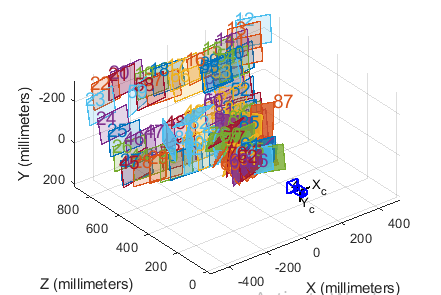
\includegraphics[width=\linewidth]{../Photos/CameraCalibration/1920x1080/calib-samples.png}\\
      {(a) Images in \Abbr{3D} space }
    \end{minipage}%
    % -----------------
    \begin{minipage}{.6\textwidth}
      \centering
      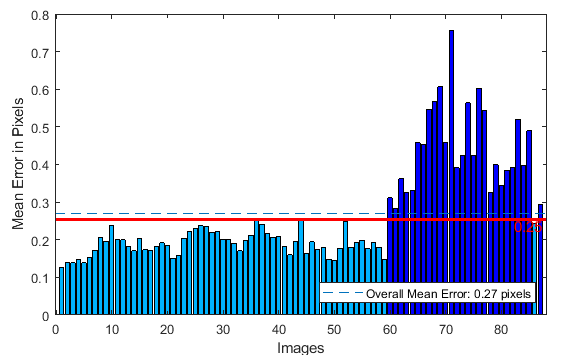
\includegraphics[width=\linewidth]{../Photos/CameraCalibration/1920x1080/calib-mean-error.png}\\
      {(b) Mean Error in pixels per image }
	\end{minipage}
	% ----------------- 
    \hfill \break
    \decoRule
    \CaptionBasedwithURL{Matlab camera toolkit} 
    \label{fig:matlab-useful-graphs}
\end{figure}

% ------------------

\subsection{Χρήση κάμερας} \label{sec:camera-usage}
Προκειμένου να λειτουργεί η κάμερα με το \Abbr{ROS}, χρειάστηκε αρχικά να συνδεθεί μέσω USB με το Raspberry Pi, ενώ χρησιμοποιήθηκε το package \textbf{usb\_cam} για την διαχείριση της. Στο launch αρχείο που δημιουργήθηκε, κατά την εκτέλεση του \textit{/usb\_cam\_node}, γίνεται επιλογή της ανάλυσης που πρόκειται να χρησιμοποιηθεί\udot όπως επίσης μέσω της παραμέτρου \textit{camera\_info\_url}, επιλέγεται το yaml αρχείο με τα χαρακτηριστικά της κάμερας που δημιουργήθηκε κατά το calibration. 

Το \textit{/usb\_cam\_node} κάνει publish στο topic \textit{/usb\_cam/image\_raw} τα περιεχόμενα της κάμερας. Το \textbf{image\_proc} είναι υπεύθυνο για το undistortion του image ώστε να μπορούν να πραγματοποιηθούν αξιόπιστες μετρήσεις.  Η επεξεργασία του stream της κάμερας γίνεται από το node με όνομα \textit{/worker\_node} που δημιουργήθηκε, το οποίο κάνει subscribe στο topic της undistorted εικόνας, μετασχηματίζει από πακέτα \Abbr{ROS} σε Mat στοιχεία - που χρησιμοποιεί το \Abbr{OpenCV},  μέσω του \textit{cv\_bridge} - και αναλαμβάνει το κομμάτι της \Abbr{CV} επεξεργασίας για της ανάγκες της εφαρμογής. 

\FigCaptLabelBasedURL{../Photos/camera-usage-ros.png}%
{ROS - camera related nodes/topics setup}%{ROS - camera related nodes/topics setup}%
{thesis-camera-nodes-topics-setup}%
<1>

Αρκετές ήταν οι φορές που υπήρχε ανάγκη (για λόγους αποσφαλμάτωσης), σε ο\-πτι\-κό feedback της \Abbr{CV} επεξεργασίας από nodes, που μπορεί να είναι διαφορετικά φυσικά μηχανήματα από αυτά που τρέχει η εφαρμογή. Πράγμα που εύκολα επιλύεται αξιοποιώντας το package \textbf{/web\_video\_server}. Αυτό είναι subscriber στο topic \textit{/usb\_\-cam/processed\_ image} (topic στο οποίο το \textit{/worker\_node} κάνει publish τα αποτελέσματα της επεξεργασίας) ώστε μέσω κάποιου browser να μπορούμε εύκολα να δούμε τα αποτελέσματα της. Η \Fig{thesis-camera-nodes-topics-setup} παρουσιάζει τα topics/nodes που αναφέρθηκαν και τον τρόπο με τον οποίο επι\-κοι\-νω\-νούν.

%----------------------------------------------------------------------

\subsection{Εντοπισμός Αντικειμένου}
Το αντικείμενο του οποίου η θέση επιλέχθηκε να προσδιοριστεί, είναι μία μπάλα - καθώς μπορεί να προσφέρει ανεξαρτήτου γωνία λήψης ίδια πληροφορία για τις διαστάσεις της - μεγέθους ανάλογη με τις μπάλες ποδοσφαίρου. 
Συνεπώς δεν μας ενδιαφέρει το orientation του αντικειμένου, παρά μόνο το location.

%----------------------------------------------------------------------

\subsubsection{Με βάση το χρώμα} \label{sec:hsv-detection-sec}

Πρώτη προσπάθεια εκτίμησης της θέσης, ήταν χρησιμοποιώντας ως σημείο αναφοράς το χρώμα της. Έχοντας επιλέξει το χρώμα της μπάλας να είναι διαφορετικό από τα περισσότερα στοιχεία της σκηνής στην οποία την καταγράφουμε, μπορούμε εύκολα να προσδιορίσουμε και την θέση του αντικειμένου στο image plane.

Συχνά οι λήψεις μίας κάμερας αναπαριστάνονται στο RGB color space, αρκετά χρήσιμο όμως είναι η χρήση του HSV για \Abbr{CV} εφαρμογές, με κύριο λόγο τον διαχωρισμό που παρέχεται μεταξύ color information και intensity στο συγκεκριμένο color space. Οπτική αναπαράσταση αυτών βρίσκεται στην \Fig{color-space}. 

\begin{figure} [H]
	\centering
	% -----------------
    \begin{minipage}{.5\textwidth}
      \centering
      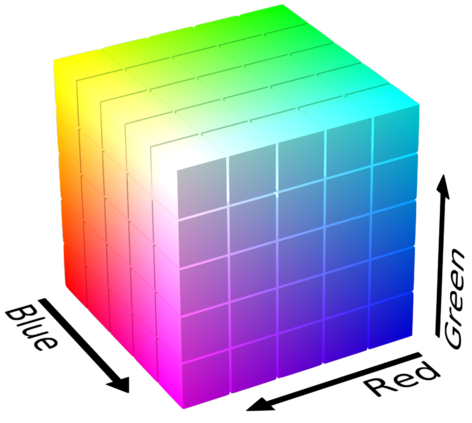
\includegraphics[width=0.5\linewidth]{../Images/Design-Implementation/rgb.png}\\
      {(a) RGB \URI{https://www.google.com/imgres?imgurl=https\%3A\%2F\%2Fqph.fs.quoracdn.net\%2Fmain-qimg-d33e22b88db273d09513f652bcb79736&imgrefurl=https\%3A\%2F\%2Fwww.quora.com\%2FWhat-are-the-differences-between-RGB-HSV-and-CIE-Lab&tbnid=XWOdefD1z2_-gM&vet=12ahUKEwjE5Iacxo_zAhW95LsIHeBlCGYQMygKegUIARCzAQ..i&docid=8mJRsf1Rk3zM_M&w=1600&h=1200&q=rgb\%20vs\%20hsv&hl=el&client=ubuntu&ved=2ahUKEwjE5Iacxo_zAhW95LsIHeBlCGYQMygKegUIARCzAQ}}
    \end{minipage}%
    % -----------------
    \begin{minipage}{.5\textwidth}
      \centering
      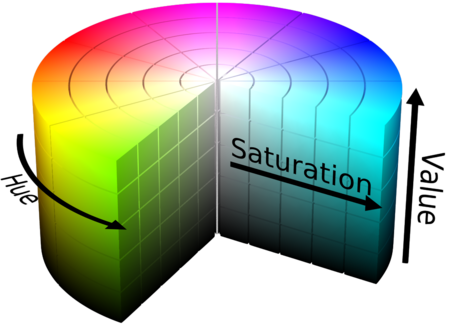
\includegraphics[width=.6\linewidth]{../Images/Design-Implementation/hsv.png}\\
      {(b) HSV \URI{https://www.google.com/imgres?imgurl=https\%3A\%2F\%2Fqph.fs.quoracdn.net\%2Fmain-qimg-7c6685f64cf5ea346a9c33be0d256a95&imgrefurl=https\%3A\%2F\%2Fwww.quora.com\%2FWhat-are-the-differences-between-RGB-HSV-and-CIE-Lab&tbnid=BwsDxAXpjI2MqM&vet=12ahUKEwjE5Iacxo_zAhW95LsIHeBlCGYQMygBegUIARCdAQ..i&docid=8mJRsf1Rk3zM_M&w=1600&h=1200&q=rgb\%20vs\%20hsv&hl=el&client=ubuntu&ved=2ahUKEwjE5Iacxo_zAhW95LsIHeBlCGYQMygBegUIARCdAQ}}
	\end{minipage}
	% -----------------
    \hfill \break
    \decoRule
    \CaptionBasedwithURL{Color Spaces} 
    \label{fig:color-space}
\end{figure}

Στον \Algo{hsv-detect} παρουσιάζεται η διαδικασία που ακολουθήθηκε προκειμένου να ε\-ντο\-πι\-στεί η μπάλα στην σκηνή με βάση το χρώμα της, στην \Fig{hsv-procedure} όμοια η επεξεργασία, ενώ στην \Fig{balls-detection-color} ε\-μφα\-νί\-ζο\-νται τα αποτελέσματα από το κάθε επίπεδο επεξεργασίας.

% ALGORITHM
\begin{algorithm}[H]
	\caption[HSV (color based) ball detection]{HSV (color based) ball detection}\label{alg:hsv-detect}
	\begin{algorithmic}[1]
		\Statex{{\bf procedure} detectBall}{}
            \State Define preferable color limit HSV values
            \For{\texttt{Each frame of the video/stream}}
                \State Get frame
                \State Remove high frequencies from it
                \State Convert frame from RGB to HSV color space
                \State Choose only pixels that are in between preferable color limit values 
                \State Find bounding box of mask (threshold image)
            \EndFor
	\end{algorithmic}
\end{algorithm}

\FigCaptLabelBasedURL{../Photos/HSV-Procedure.png}%
{Επεξεργασία για ανίχνευση με βάση το χρώμα}%{Detect balls based on their shape}%
{hsv-procedure}%
<0.8>

\FigCaptLabelBasedURL{../Photos/thesis-hsv.png}%
{Ανίχνευση μπάλας με βάση το χρώμα}%{Detect balls based on their color}%
{balls-detection-color}%
<0.9>

Ένα μεγάλο μέρος των \Abbr{CV} εφαρμογών περιλαμβάνει ως διαδικασίες επεξεργασίας το να γίνεται convolution ή cross-correlation\footnote{Η διαφορά μεταξύ του convolution και του cross-correlation, είναι ότι στο convolution ο kernel αναστρέφεται} ενός kernel με τα pixel της εικόνας. Αυτή η διαδικασία - που για το convolution περιγράφεται μαθηματικά από την εξίσωση \EqNum{cross-correlation} και οπτικά από την \Fig{convolution-example} - έχει ποικίλες εφαρμογές οι οποίες διαχωρίζονται με βάση την επιλογή του kernel. Μία εξ' αυτών είναι για λόγους smoothing, που στην συγκεκριμένη περίπτωση περιλαμβάνει σημαντική διαδικασία του preprocessing, καθώς με αυτόν τον τρόπο μειώνουμε την ποσότητα των υψηλών συχνοτήτων συνεπώς και τον θόρυβο στην εικόνα.

\begin{gather}
	O[i,j] = k * I = \sum_{u=-k}^{k} \sum_{v=-k}^{k} k[u,v]I[i-u,j-v] \label{eq:cross-correlation}
\end{gather}

\FigCaptLabelBasedURL{../Images/Design-Implementation/cross-correlation.png}%
{Convolution παράδειγμα}%{Convolution Example}%
{convolution-example}%
<0.5>%
(http://intellabs.github.io/RiverTrail/tutorial/)

Συγκεκριμένα χρησιμοποιήθηκε Gaussian μορφής kernel το οποίο παρέχει πιο φυσικής μορφής blur, και αφού έγινε το transform σε HSV επιλέχθηκαν μόνο τα pixel των οποίων οι τιμές ήταν αποδεκτές. Δύο μειονεκτήματα της συγκεκριμένης μεθόδου είναι ότι τα αποτελέσματα μεταβάλλονται σημαντικά ανάλογα τις συνθήκες φωτισμού, ακόμα και σε επίπεδο που για ίδια thresholds να μην γίνεται ανίχνευση του α\-ντι\-κει\-μέ\-νου. Όπως επίσης, αν το χρώμα του αντικειμένου δεν επιλεχθεί κατάλληλα - παράδειγμα στην \Fig{balls-detection-color} για τις άσπρες μπάλες - το αντικείμενο τελικά να μην μπορεί να εντοπιστεί. 

%----------------------------------------------------------------------

\subsubsection{Με βάση το σχήμα}

Στη δεύτερη προσπάθεια εντοπισμού της μπάλας, χρησιμοποιήθηκε η πληροφορία του σχήματος της, καθώς η προβολή που καταγράφει η κάμερα για αυτή, δεν είναι παρά ένας κύκλος. Με όμοιο τρόπο στον \Algo{hough-detect} παρουσιάζεται σε ψευδοκώδικα η διαδικασία, στην \Fig{hsv-procedure} όμοια η επεξεργασία, ενώ στην \Fig{balls-detection-shape} τα αποτελέσματα στο κάθε phase.

% ALGORITHM
\begin{algorithm}[H]
	\caption[Hough circle (shape based) ball detection]{Hough circle (shape based) ball detection}\label{alg:hough-detect}
	\begin{algorithmic}[1]
		\Statex{{\bf procedure} HoughdetectBall}{}
            \For{\texttt{Each frame of the video/stream}}
                \State Get frame
                \State Convert frame from RGB to Grayscale
                \State Remove high frequencies from the frame
                \State Use Hough Transform principle to detect circles in image 
            \EndFor
	\end{algorithmic}
\end{algorithm}

\FigCaptLabelBasedURL{../Photos/Hough-Procedure.png}%
{Επεξεργασία για ανίχνευση με βάση το σχήμα}%{Detect balls based on their shape}%
{hough-procedure}%
<0.8>

\FigCaptLabelBasedURL{../Photos/thesis-hough.png}%
{Ανίχνευση μπάλας με βάση το σχήμα}%{Detect balls based on their shape}%
{balls-detection-shape}%
<0.8>

Για τον εντοπισμό του κυκλικού σχήματος της μπάλας χρησιμοποιήθηκε o Hough Transform for circles detection.
Ο τρόπος με τον οποίο λειτουργεί ο Hough Transform είναι να μετασχηματίζει το circle localization πρόβλημα σε ένα voting πρόβλημα.
Είσοδος στον αλγόριθμο Hough είναι τα edges ενός image, και έξοδος είναι η θέσεις των κύκλων.

Η απλούστερη περίπτωση του Hough Transform είναι σε μία εικόνα να κάνουμε localize έναν κύκλο με γνωστό radius r, όπως παρουσιάζεται στην \Fig{hough-tranform-examples} (a). Σε αυτήν την περίπτωση για κάθε στοιχειώδες σημείο (x,y) των edges δημιουργούμε στο Hough space έναν κύκλο ακτίνας r με κέντρο (x,y). Αφού γίνει αυτή η διαδικασία για κάθε σημείο των edges, το σημείο στο hough space (εναλλακτικό όνομα accumulator) με τα περισσότερα votes - σημείο χρώματος πράσινο στην \Fig{hough-tranform-examples} (a) - είναι τελικά και το κέντρο του κύκλου.

\begin{figure} [H]
	\centering
	% -----------------
    \begin{minipage}{.5\textwidth}
      \centering
      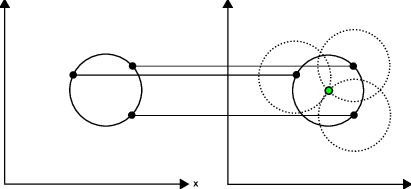
\includegraphics[width=\linewidth]{../Images/Design-Implementation/circle-hough-2d.png}\\
      {(a) Hough space for known radius \URI{https://www.researchgate.net/figure/The-circular-Hough-transform_fig1_242103081}}
    \end{minipage}%
    % -----------------
    \begin{minipage}{.5\textwidth}
      \centering
      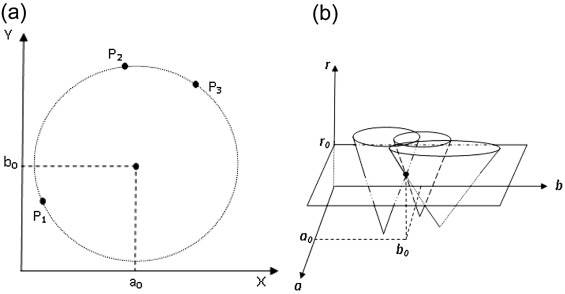
\includegraphics[width=.9\linewidth]{../Images/Design-Implementation/circle-hough-3d.jpg}\\
      {(b) Hough space for unknown radius \URI{https://www.sciencedirect.com/science/article/abs/pii/S0030402616316175}}
	\end{minipage}
	% -----------------
    \hfill \break
    \decoRule
    \CaptionBasedwithURL{Circle Hough Transform} 
    \label{fig:hough-tranform-examples}
\end{figure}

Η πιο σύνθετη περίπτωση - \Fig{hough-tranform-examples} (b) - είναι όταν δεν γνωρίζουμε την ακτίνα του κύκλου που αναζητούμε στην σκηνή, σε αυτήν την περίπτωση επαναλαμβάνουμε την παραπάνω διαδικασία για διαφορετικές τιμές ακτίνων, με αποτέλεσμα στο Hough space να δημιουργήσουμε κώνους αντί για κύκλους. Ενώ, οι συντεταγμένες του σημείου με τα περισσότερα votes στον accumulator, σε αυτήν την περίπτωση μας προσδιορίζουν τις συντεταγμένες του κέντρου του κύκλου μαζί με την ακτίνα του.

\subsubsection{Εναλλακτικές προσεγγίσεις}
Υπάρχουν αρκετές εναλλακτικές μεθοδολογίες που θα μπορούσαν επίσης να χρησιμοποιηθούν για το localization του object στο image plane, όπως το background extraction, tracking ενός object που γίνεται defined στην αρχή της λειτουργίας ή ακόμα και machine learning based προσεγγίσεις. 

Ένας επιπλέον, σύμφωνα με αυτά, τρόπος που έγινε προσπάθεια να εντοπιστεί - δυ\-στυ\-χώς χωρίς θετικά αποτελέσματα - η μπάλα στην εικόνα, είναι μέσω της τεχνικής haar cascade classifier \cite{opencv-haar-cascade} η οποία αποτελεί μία weak machine learning τακτική, που έχει χρησιμοποιηθεί στο παρελθόν σε ανίχνευση της μπάλας σε εφαρμογές όπως για RoboCup \cite{opencv-haar-cascade-robot1} \cite{opencv-haar-cascade-robot2}.

Πρακτικά, σε αυτή χρησιμοποιούνται δύο dataset, ένα θετικό στο οποίο παρουσιάζεται το αντικείμενο ενδιαφέροντος που θέλουμε να εκπαιδεύσουμε το μοντέλο να αναγνωρίζει και ένα αρνητικό στο οποίο δεν βρίσκεται. Για αυτόν τον λόγο, στην προσπάθεια να δημιουργηθεί ένα παρόμοιο μοντέλο για την συγκεκριμένη εφαρμογή πάρθηκαν πάνω από 1000 φωτογραφίες της μπάλας όπως παρουσιάζονται στην \Fig{haar-cascade-dataset-example} ενώ επίσης υπήρξαν και περίπου 4000 φωτογραφίες για το αρνητικό dataset.

\FigCaptLabelBasedURL{../Images/Design-Implementation/haar-cascade-clas-input-sample.jpg} %
{Παράδειγμα από το θετικό dataset που δημιουργήθηκε, για να γίνει train το μοντέλο του haar cascade.} %
{haar-cascade-dataset-example} %
<0.8>

%----------------------------------------------------------------------

\subsection{Εκτίμηση απόστασης}
Αφού είχε εντοπιστεί η θέση του αντικείμενο στην εικόνα καθώς και η ακτίνα του σε pixel, μπορούσε να υπολογιστεί και η απόσταση του από την κάμερα. 
Για τον υπολογισμό της απόστασης της μπάλας, χρησιμοποιείται ως κύρια αρχή ο φο\-ρμα\-λι\-σμός που περιγράφηκε στη \Sect{theo-structure-from-reference} - \Equa{distance-from-object} - η οποία χρειάζεται να μετασχηματιστεί ώστε σαν είσοδο να χρησιμοποιεί πλήθος pixel και όχι mm, συνεπώς μέσω της εξίσωσης \EqNum{distance-from-object-pixels} μπορούμε να υπολογίσουμε την απόσταση που μας ενδιαφέρει, υπολογίζοντας μόνο το πλήθος των pixel που καταλαμβάνει στην εικόνα το αντικείμενο \cite{calculate-distance-stackexchange} \cite{calculate-distance-or-size-of-an-objectin-a-photo-image}.

\begin{align}
	\textrm{Distance (m)} &= \frac{\textrm{$f$ (mm)}\; x\;\textrm{Object real size(m)}\; x\; \textrm{Image size(pixels)}}{\textrm{Object size on sensor (pixels)}\; x\; \textrm{Sensor size(mm)}} \label{eq:distance-from-object-pixels}
\end{align}

%----------------------------------------------------------------------

\subsection{Εκτίμηση γωνίας}
Για την εκτίμηση γωνίας ως προς τον x και y άξονα του image plane σε μία calibrated κάμερα μπορεί να χρησιμοποιηθεί η \Equa{angle-from-object-center-pixels}, η οποία είναι στην πραγματικότητα υλοποίηση απλής μεθόδου των τριών με βάση το Field of View (\Abbr{FOV}) μίας κάμερας. Σε περίπτωση που δεν γνωρίζουμε το \Abbr{FOV} μπορεί να υπολογιστεί ως προς την συσχέτιση του Angular Field of View (\Abbr{AFOV}) με το Focal length
της κάμερας, αυτή η εξάρτηση παρουσιάζεται οπτικά στην \Fig{focal-length-fov} και μαθηματικά στην \Equa{afov-focal-length} \cite{afov-focal-length-rela} και στην συνέχεια μέσω της σχέσης \EqNum{afov-to-fov} μπορούμε να μεταβούμε από το ένα στο άλλο. 

\begin{align}
	\textrm{Angle (\si{\degree})} &= \frac{\textrm{FOV(\si{\degree})}\; x\;\textrm{distance from origin (pixel)}}{\textrm{image length(pixel)}} \label{eq:angle-from-object-center-pixels}
\end{align}

\begin{align}
	\textrm{AFOV(\si{\radian})} &= 2\tan^{-1}{\frac{\textrm{image length(mm)}}{2\; x\;\textrm{focal length(mm)}}} \label{eq:afov-focal-length}
\end{align}

\begin{align}
	\textrm{FOV(\si{\degree})} &= \frac{\textrm{AFOV(\si{\radian})}\; x\;\textrm{180}}{\pi} \label{eq:afov-to-fov}
\end{align}

\FigCaptLabelBasedURL{../Images/Design-Implementation/fov-focal-length.png} %
{Συσχέτιση AFOV με focal length} %
{focal-length-fov} %
<0.8>
(https://www.princetoninstruments.com/learn/camera-fundamentals/field-of-view-and-angular-field-of-view)

%----------------------------------------------------------------------

\section{Διαμοιρασμός μηνυμάτων}
Έχοντας εντοπίσει σε κάθε worker node το αντικείμενο και εκτιμήσει μέσω των παραπάνω εξισώσεων τις πληροφορίες που μας ενδιαφέρουν, επόμενο βήμα είναι ο διαμοιρασμός των μηνυμάτων με κατεύθυνση το master node, για την εκτίμηση της θέσης. Προκειμένου να περαστεί πληροφορία μέσα στο δίκτυο με node, χρειάστηκε να δημιουργηθούν proprietary πακέτα, στα οποία θα αποθηκεύονταν αυτές οι πληροφορίες. Συγκεκριμένα κάθε node αφού πραγματοποιήσει όλη την επεξεργασία, α\-πο\-στέ\-λλει mocap\_worker\_data πακέτα στο δίκτυο Wi-Fi όπου είναι συνδεδεμένα όλα τα nodes. Αυτά ακολουθούν την δομή που εμφανίζονται στην \Fig{proprietary-msg}, η οποία δημιουργήθηκε για τις ανάγκες του συστήματός και μέσα σε αυτή πε\-ρι\-λα\-μβά\-νο\-νται πληροφορίες σχετικά με τον σειριακό αριθμό του node, την θέση του, τα χα\-ρα\-κτη\-ρι\-στι\-κά της κάμερας του, επίσης πληροφορία για κάθε αντικείμενο που ανιχνεύτηκε καθώς και για τον συγχρονισμό των πακέτων. 

% Codeshare -> eclipse
% mocap_worker_data
% ├── header
% ├── timestamp
% ├── nodeID
% ├── master_time
% │   ├── header
% │   ├── ros_time
% │   ├── internal_time
% │   └── packet_id
% ├── obj_pose
% │   ├── x
% │   ├── y
% │   ├── z
% │   ├── roll
% │   ├── pitch
% │   └── yaw
% ├── camera_params
% │   ├── objectsRealSizeInMeter
% │   ├── imageHeightInPixels
% │   ├── imageWidthInPixels
% │   ├── XFieldOfViewInAngles
% │   ├── YFieldOfViewInAngles                    
% │   ├── XfocalLengthInMillimeters
% │   ├── YfocalLengthInMillimeters
% │   ├── XsensorSizeInMillimeters
% │   └── YsensorSizeInMillimeters
% └── detected_ball_data[]
%     ├── id
%     ├── color
%     ├── distance_from_camera
%     ├── image_plane_r
%     ├── image_plane_x
%     ├── image_plane_y
%     ├── xangle
%     └── ynagle
\FigCaptLabelBasedURL{../Images/Design-Implementation/ros-msgs-hier.png} %
{Η δομή του μηνύματος που αποστέλλει κάθε node} %{Proprietary message send structure} %
{proprietary-msg} %
<0.38>

%----------------------------------------------------------------------

\section{Συγχρονισμός μηνυμάτων}
Σημαντικό είναι η επίτευξη συγχρονισμού μεταξύ των μηνυμάτων που α\-πο\-στέ\-λλο\-νται. Για αυτό ο master node προγραμματίστηκε να κάνει broadcast, τακτικά, πακέτα τύπου master\_time (βλ. μέρος του πακέτου της \Fig{proprietary-msg}) με το ρολόι το οποίο έχει αυτός. Όταν τα worker nodes λάβουν αυτήν την πληροφορία, την αποθηκεύουν σε εσωτερικό buffer, πραγματοποιούν το detection και localization και στα mocap\_worker\_data που στέλνουν πίσω, συμπεριλαμβάνουν και αυτήν την πληροφορία. Με αυτόν τον τρόπο ο συγχρονισμός των πακέτων γίνεται με βάση το ρολόι του master, ο οποίος είναι και αυτός που επεξεργάζεται και τα δεδομένα. Η \Fig{sync-sequence-diagram} προσεγγίζει σε abstract μορφή αυτήν την επικοινωνία. Με βάση την θεώρηση που έγινε για την σχεδίαση του συστήματος, ότι τόσο το αντικείμενο όσο και τα nodes κινούνται με μικρές ταχύτητες - άρα σε μικρό χρονικό διάστημα - δεν υπάρχει μεγάλη μεταβολή της θέσης, επιλέχθηκε ο master να κάνει broadcast τα πακέτα συγχρονισμού με συχνότητα 2Hz, ενώ τα nodes αποστέλλουν πληροφορία στο master με συχνότητα 10Hz. Επίσης οι valid εκτιμήσεις θέσεις της μπάλας οι οποίες γίνονται broadcast στο σύστημα από το master, γίνονται με συχνότητα 2Hz.  

\FigCaptLabelBasedURL{../Photos/synchronization.png} %
{High level sequence diagram για τον συγχρονισμό των πακέτων} %{Proprietary message send structure} %
{sync-sequence-diagram} %
<1>

%----------------------------------------------------------------------

\section{Εντοπισμός θέσης αντικειμένου}\label{sec:implementation-obj-mult}
Για να εντοπιστεί τελικά στον τρισδιάστατο χώρο το αντικείμενο, χρησιμοποιείται η αρχή λειτουργίας του Trilateration αλγορίθμου, που αναφέρθηκε στη \Sect{trilateration}. Που όμως επειδή είναι στον \Abbr{3D} χώρο, στον οποίο χρειαζόμαστε τουλάχιστον 4 κόμβους για τον καθορισμό της θέσης, ονομάζεται Multilateration \ref{sec:Multilateration}. Όπως αναφέρθηκε και στη \Sect{trilateration}, πρακτικά προσπαθούμε για τις εξισώσεις \EqNum{multilateration-pha1} με γνωστά τα $(x_i, y_i, z_i)$ και $r_i$ να βρούμε τα $(x,y,z)$. 
 
\begin{align}
	(x-x_1)^2 + (y-y_1)^2 + (z-z_1)^2 &= r_1^2 \label{eq:multilateration-pha1} \\ 
	(x-x_2)^2 + (y-y_2)^2 + (z-z_2)^2 &= r_2^2 \nonumber \\
	(x-x_3)^2 + (y-y_3)^2 + (z-z_3)^2 &= r_3^2 \nonumber \\
	(x-x_4)^2 + (y-y_4)^2 + (z-z_4)^2 &= r_4^2 \nonumber 
\end{align}

Ένας τρόπος προσέγγισης, για επίλυση των εξισώσεων \EqNum{multilateration-pha1} είναι να τις αναλύσουμε στις \EqNum{multilateration-pha2} 
και από εκεί να έχουμε να λύσουμε το γραμμικό σύστημα πινάκων που περιγράφεται στην \EqNum{multilateration-linear-system} \cite{Multilateration-Solution}.

\begin{align}
	(x^2+y^2+z^2) - 2x_1x - 2y_1y - 2z_1z &= r_1^2 - x_1^2 - y_1^2 - z_1^2 \label{eq:multilateration-pha2} \\ 
	(x^2+y^2+z^2) - 2x_2x - 2y_2y - 2z_2z &= r_2^2 - x_2^2 - y_2^2 - z_2^2 \nonumber \\
	(x^2+y^2+z^2) - 2x_3x - 2y_3y - 2z_3z &= r_3^2 - x_3^2 - y_3^2 - z_3^2 \nonumber \\
	(x^2+y^2+z^2) - 2x_4x - 2y_4y - 2z_4z &= r_4^2 - x_4^2 - y_4^2 - z_4^2 \nonumber
\end{align}


\begin{align}
	A = \begin{bmatrix} 1 && -2x_1 && -2y_1 && -2z_1 \\ 1 && -2x_2 && -2y_2 && -2z_2 \\ 1 && -2x_3 && -2y_3 && -2z_3 \\ 1 && -2x_4 && -2y_4 && -2z_4 \\\end{bmatrix} \nonumber \quad
	X = \begin{bmatrix} x^2+y^2+z^2 \\x \\ y \\ z \end{bmatrix} \nonumber \quad
	B = \begin{bmatrix} r_1^2 - x_1^2 - y_1^2 - z_1^2 \\ r_2^2 - x_2^2 - y_2^2 - z_2^2 \\ r_3^2 - x_3^2 - y_3^2 - z_3^2 \\ r_4^2 - x_4^2 - y_4^2 - z_4^2 \end{bmatrix} \nonumber
\end{align}

\begin{align}
	AX = B \label{eq:multilateration-linear-system}
\end{align}

Θετικό με την συγκεκριμένη μέθοδο προσέγγισης - μέσω των εξισώσεων \EqNum{multilateration-pha2} - είναι ότι εύκολα το σύστημα μπορεί να γίνει scale καθώς η κάθε στήλη των πινάκων εξαρτάται μόνο από δεδομένα ενός μεμονωμένου node. Άρα παρόλο που στην συ\-γκε\-κρι\-μένη διπλωματική κάνουμε πειράματα για δεδομένα τεσσάρων θέσεων, με την ίδια ευκολία θα μπορούμε να ήταν και για N όπου $N>4$.

Η υλοποίηση του συγκεκριμένου αλγορίθμου πραγματοποιήθηκε με την βοήθεια της βιβλιοθήκης Eigen, η οποία αποτελεί και την προτεινόμενη για το ROS βιβλιοθήκη για διαχείριση πινάκων και υπολογισμών σε linear math. 



%----------------------------------------------------------------------
\section{Τρισδιάστατη απεικόνιση}
Για την τρισδιάστατη απεικόνιση των δεδομένων που συλλέχθηκαν κατά την διάρκεια των πειραμάτων - που περιγράφονται στο επόμενο κεφάλαιο - χρησιμοποιήθηκε το εργαλείο Matlab, μέσω του οποίου έγιναν οι περισσότερες γραφικές. Σημαντική όμως είναι και η βοήθεια του πακέτου RViz του ROS, το οποίο σε real time χρόνο μπορεί να οπτικοποιήσει δεδομένα.

%----------------------------------------------------------------------

\section{Επαλήθευση ID του detected object}\label{sec:id-estimation}
Για λόγους πληρότητας, καθώς και επαλήθευσης του detection, ως τελευταίο σκέλος του συστήματος, προτείνεται ένας τρόπος ώστε να μπορεί να αποδοθεί ID στο αντικείμενο το οποίο ανιχνεύτηκε. Το ID μπορεί να χρησιμοποιηθεί για την πραγματοποίηση localization συγκεκριμένου αντικείμενου - σε περίπτωση που υπάρχουν περισσότερα από ένα στο scene. 

Ο τρόπος που προσεγγίστηκε το πρόβλημα είναι με την ανίχνευση ενός γεγονότος στο stream της κάμερας. Συγκεκριμένα, αφού ανιχνευτεί το αντικείμενο όπως επεξηγήθηκε στο παρόν κεφάλαιο, επιλέγεται εσωτερικά των εξωτερικών διαστάσεων του αντικειμένου να φωτοβολεί ένα led για τον προσδιορισμό του γεγονός αναφοράς. Αυτό μπορεί να είναι περιοδικό είτε κωδικοποιημένο - βλ. \Fig{id-calc} - ώστε ο προσδιορισμός του ID να μετατραπεί σε ένα χρονικό πρόβλημα.

Ακολουθείται παρόμοια διαδικασία όπως περιγράφηκε στη \Sect{hsv-detection-sec}, όμως για το led που βρίσκεται εσωτερικά του bounding box που περικλείει η μπάλα. Πλέον το εμβαδόν του bounding box για το led, όταν δεν είναι αναμμένο αυτό\udot είναι μηδενικό, ενώ σε αντίθετη περίπτωση έχει μία μη μηδενική τιμή. Με τον μετασχηματισμό του προβλήματος, πλέον, μετρώντας τον χρόνο ενδιάμεσα μηδενικών τιμών για το εμβαδόν του bounding box που δημιουργείται λόγο του led, είναι εφικτός ο προσδιορισμός μοναδικού ID.

\begin{figure} [H]
	\centering
	% -----------------
    \begin{minipage}{.5\textwidth}
      \centering
      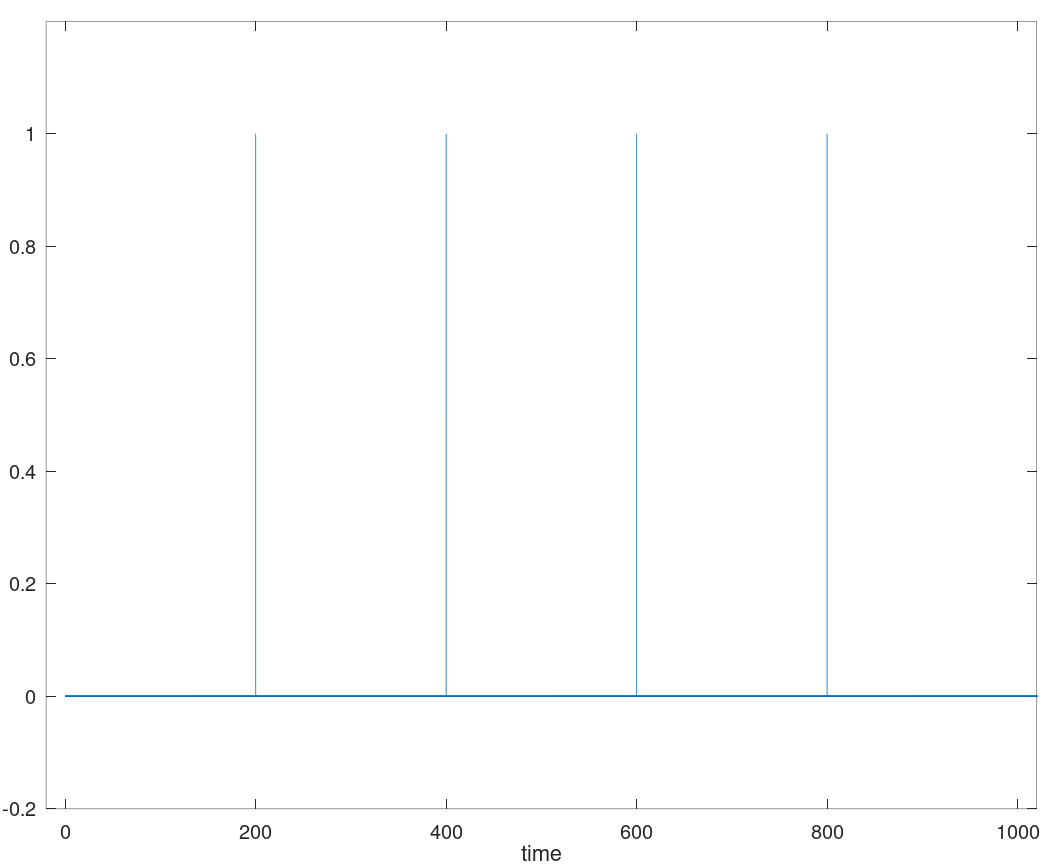
\includegraphics[width=0.9\linewidth]{../Images/Experiments-Results/freq-id.png}\\
      {(a) Mε βάση την συχνότητα}
    \end{minipage}%
    % -----------------
    \begin{minipage}{.5\textwidth}
      \centering
      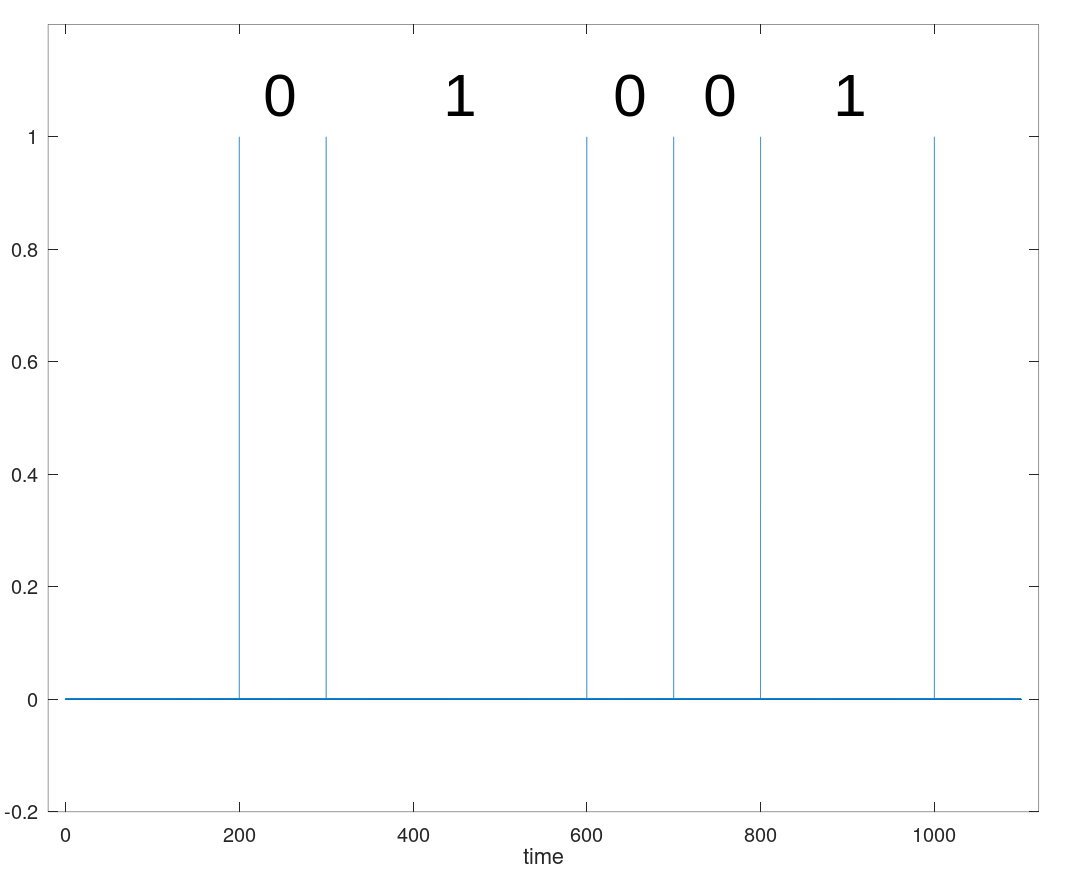
\includegraphics[width=.9\linewidth]{../Images/Experiments-Results/enco-id.png}\\
      {(b) Mε βάση κωδικοποίηση}
	  \end{minipage}
% -----------------
    \hfill \break
    \decoRule
    \caption[Παραδείγματα προσεγγίσεων καθορισμού του ID]{Παραδείγματα προσεγγίσεων καθορισμού του ID}%\CaptionBasedwithURL{Possible Embedded Linux Systems} 
    \label{fig:id-calc}
\end{figure}

Στην συγκεκριμένη εργασία επιλέχθηκε ο προσδιορισμός να γίνει με βάση την σταθερή συχνότητα με την οποία κάνει blink το led.

%----------------------------------------------------------------------

